\documentclass{standalone}

\usepackage{tikz}

\usetikzlibrary{positioning, chains, shapes.geometric, fit, shapes, arrows.meta, calc}

\begin{document}

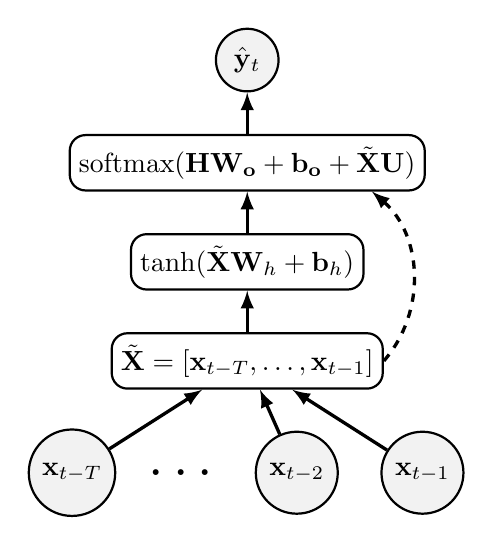
\begin{tikzpicture}[
    >=LaTeX, % Use default LaTeX arrows
    % Styles 
    layer/.style={
        rectangle,
        fill=white!10,
        rounded corners=2mm,
        minimum height=2em,
        minimum width=3em,
        draw,
        thick
    },
    input/.style={ % Input or output node
        circle,
        minimum width=2.25em,
        draw,
        fill=gray!10,
        thick
    },
    arrow/.style={
        -latex,
        very thick
    },
    residual/.style={
        arrow,
        dashed
    }
]

    % Inputs
    \node[input] (xT) {$\mathbf{x}_{t-T}$};
    \node[input, right=5em of xT] (x2) {$\mathbf{x}_{t-2}$};
    \node[input, right=1.5em of x2] (x1) {$\mathbf{x}_{t-1}$};

    % Layers
    \node[layer, above=3em of $(x1)!0.5!(xT)$] (hidden) {$\tilde{\mathbf{X}} = [\mathbf{x}_{t-T}, \dots, \mathbf{x}_{t-1}]$};
    \node[layer, above=1.5em of hidden] (ff) {$\tanh(\tilde{\mathbf{X}}\mathbf{W}_h + \mathbf{b}_h)$};
    \node[layer, above=1.5em of ff] (linear) {softmax$(\mathbf{\mathbf{H}\mathbf{W}_o + \mathbf{b}_o} + \tilde{\mathbf{X}}\mathbf{U})$};

    % Outputs
    \node[input, above=1.5em of linear] (output) {$\hat{\mathbf{y}}_t$};

    % Continuation dots
    \path (xT) -- (x2) node[midway, scale=2] {\dots};

    % Connections
    \foreach \i in {x1, x2, xT} {
        \draw[arrow] (\i) -- (hidden);
    }
    \draw[arrow] (hidden) -- (ff);
    \draw[arrow] (ff) -- (linear);
    \draw[arrow] (linear) -- (output);

    % Residual connections
    \draw[residual] (hidden.east) to[bend right=45] (linear.347);
\end{tikzpicture}

\end{document}
